\chapter{Análisis y diseño}\label{chp:introduccion}

En este capítulo se describe el análisis y el diseño del trabajo propuesto para
la recolección, clasificación de noticias y el entorno web.

\section{Requisitos funcionales}
\begin{itemize}
  \item RF1: El sistema debe recolectar noticias de forma automática en la internet
  \item RF2: El sistema debe clasificar las noticias recolectadas deacuerdo a su contenido
  \item RF3: El sistema debe permitir filtrar las noticias deacuerdo a su fecha de publicación
  \item RF4: El sistema debe mostrar las noticias recolectadas y clasificadas al usuario en un entorno web
  \item RF5: Cada noticia mostrada debe contener un hipervínculo que rediriga al usuario a su sitio de origen 
  \item RNF6:      

\end{itemize}

\section{Requisitos No funcionales}
\begin{itemize}
\section{Estructura del Documento}
  \item RNF1: La clasificación de una noticia no debe tardar mas de un segundo
  \item RNF2: Las noticias recolectads deberán tener un mínimo de 180 palabras en
  ellas
  \item RNF3: El sistema 

\end{itemize}



\section{Reglas de negocio}
\begin{itemize}
  \item RDN1: La notica debe tener almenos 180 palabras
  \item RDN2: Las noticias deben estar redactadas en lenguaje español
\end{itemize}
  %--------------------------Casos de uso -------------------------%

\newpage
\section{Casos de uso}


\subsection{Diagrama de casos de uso}
La figura \ref{fig:DCU} muestra el diagrama de casos de uso implementado en el sistema.

\begin{figure}
  \centering
  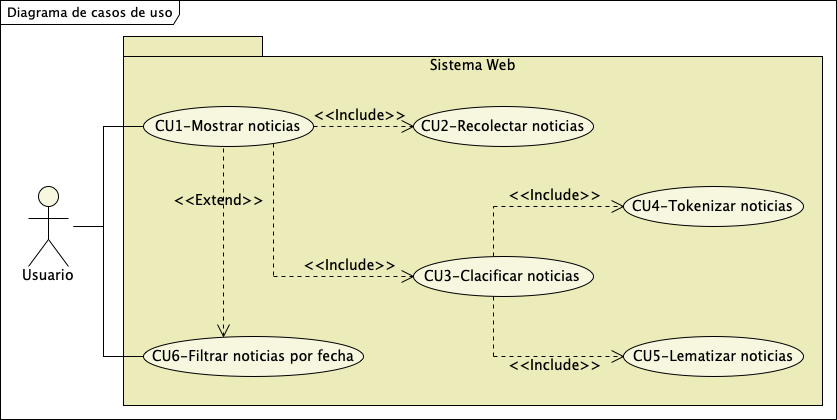
\includegraphics[scale=.5]{imagenes/Diagramas/CasosDeuso}
  \caption{Diagrama de casos de uso}
  \label{fig:DCU}
\end{figure}


\subsection{CU-1 Recolectar noticias}

\Large{\textbf{Resumen}}\\\\
\footnotesize{Texto}\\

\Large{\textbf{Descripción}}\\
\footnotesize{} 

\begin{tabular}{|l|l|}
	\hline
	\multicolumn{1}{| >{\columncolor{black}}l|}{ \textcolor{myWhite}{\textbf{Caso de uso: }} }&
	\multicolumn{1}{| >{\columncolor{black}}l|}{ \textcolor{myWhite}{CU-1 Recolectar noticias} }\\
	\hline
	\textbf{Actor:} & 	Lorem Ipsum	\\
	\hline
	\textbf{Propósito:} & Lorem Ipsum \\
	\hline
	\textbf{Entradas:} & Lorem Ipsum \\
	\hline
	\textbf{Salidas:} & Lorem Ipsum\\
	\hline
	\textbf{Precondición:} & Lorem Ipsum \\
	\hline
	\textbf{Postcondiciones:} & Lorem Ipsum \\
	\hline
	\textbf{Reglas de negocio:} & Lorem Ipsum \\
	\hline
	\textbf{Errores:} & Lorem Ipsum \\
	\hline
	\textbf{Autor:} & Lorem Ipsum \\
	\hline
\end{tabular}\\\\

%--------------------Trayectoria Principal-----------%
\Large{\textbf{Trayectorias del caso de uso}}\\\\
\large{Trayectoria principal}\\
\footnotesize{} 

	
	

\begin{enumerate}[1.]
	\item \actor lorem ipsum
	\item \sistema lorem ipsum
	\item \sistema lorem ipsum
	\item \sistema lorem ipsum
	\item \finCU	

\end{enumerate}


%--------------------trayectoria Alternatia A---------%
\normalsize{Trayectoria Alternativa A:}\\\footnotesize{}
\textbf{Condición:} \textit{Se escribe la condición}

\begin{enumerate}[{A-}1.]
	\item \actor lorem ipsum
	\item \sistema lorem ipsum
	\item \finTA	

\end{enumerate}


%--------------------trayectoria Alternatia b---------%
\normalsize{Trayectoria Alternativa B:}\\
\footnotesize{} 
\textbf{Condición:} \textit{Se escribe la condición}

\begin{enumerate}[{B-}1.]
	\item \actor lorem ipsum
	\item \sistema lorem ipsum
	\item \finTA	

\end{enumerate}



\Large{\textbf{Puntos de extensión}}\\\\\footnotesize{}

\textbf{Causa de la extensión:} Lorem ipsum\\
\textbf{Región de la trayectorioa:} Lorem ipsum\\
\textbf{Extiende a :} Lorem ipsum\\\\

\textbf{Causa de la extensión:} Lorem ipsum\\
\textbf{Región de la trayectorioa:} Lorem ipsum\\
\textbf{Extiende a :} Lorem ipsum\\

\newpage
\input{Capitulos/CasosDeUso/cu2-clasificarNoticia}
\newpage
\input{Capitulos/CasosDeUso/cu3-mostrarNoticia}
\newpage
\input{Capitulos/CasosDeUso/cu4-FiltrarNoticiaFecha}
\newpage

  %--------------------------Descripción de pantallas ------------------%
\section{Pantallas}

\input{Capitulos/CasosDeUso/DescripcionPantallas/ui1-inicio}
\newpage
\subsection{UI2-Sección deportes}

\Large{\textbf{Objetivo}}\\\\
\normalsize{Texto}\\



\Large{\textbf{Descripción}}\\
\normalsize{Texto}\\


\Large{\textbf{Comandos}}\\
\normalsize{}

\begin{itemize}
	\item Lorem ipsum
	\item Lorem ipsum
	\item Lorem ipsum
\end{itemize}

\Large{\textbf{Referencia}}\\\\
\normalsize{Nombre Caso de uso}

\begin{figure}
  \centering
	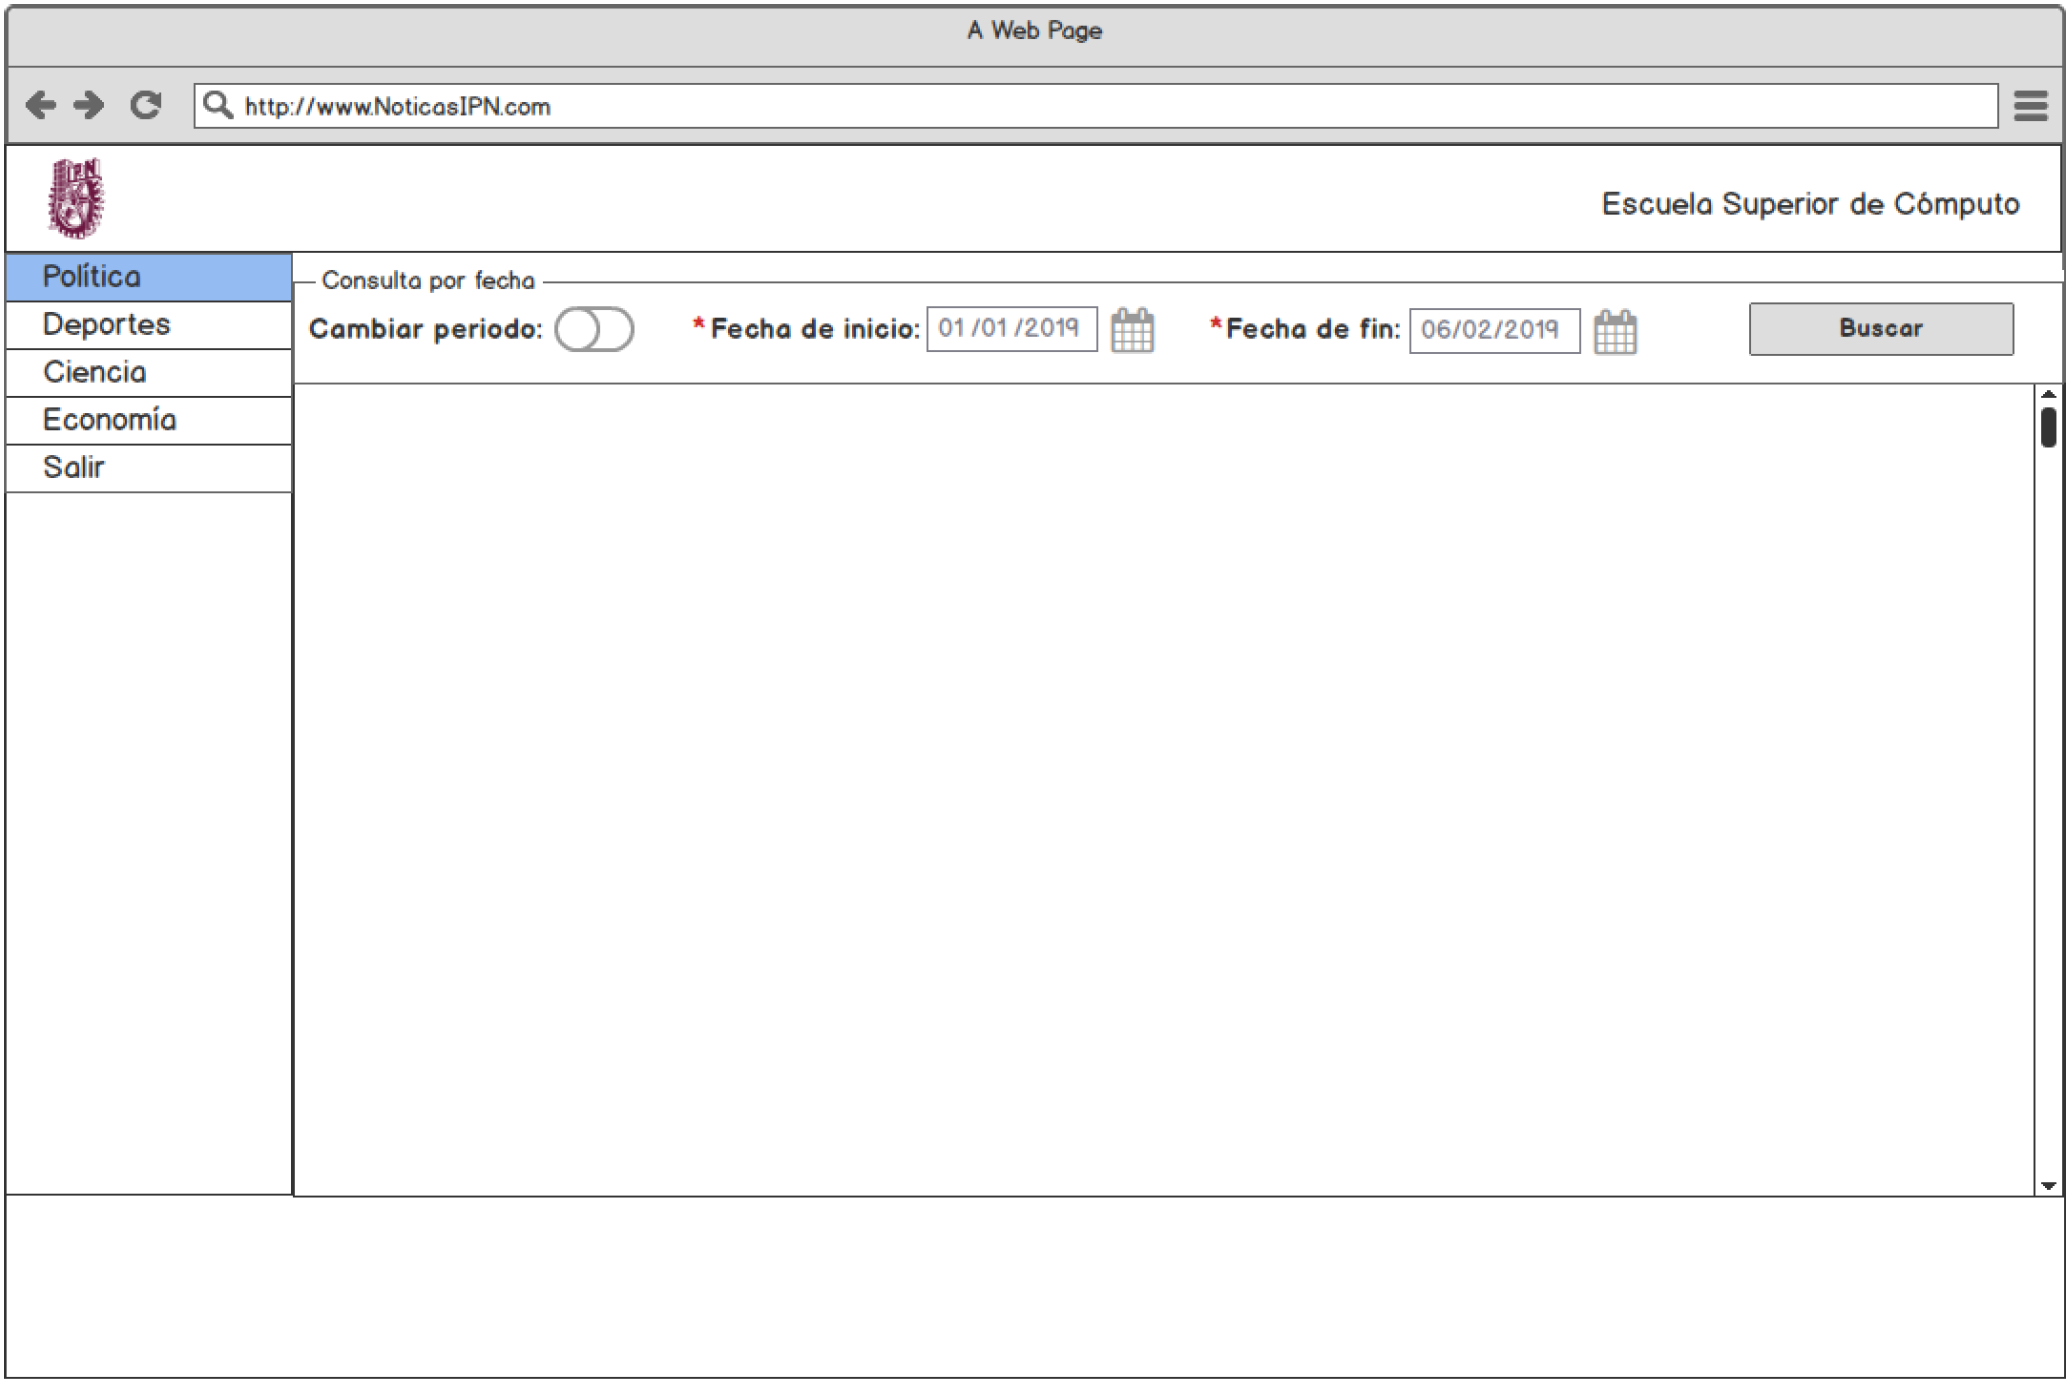
\includegraphics[scale=.3]{imagenes/Pantallas/UI2}
  \caption{Pantalla IU2-Sección deportes}
  \label{fig:IU2}
\end{figure}
\newpage
\subsection{UI3-Busqueda por fecha}

\Large{\textbf{Objetivo}}\\\\
\normalsize{Texto}\\

	

\Large{\textbf{Descripción}}\\
\normalsize{Texto}\\



\Large{\textbf{Comandos}}\\
\normalsize{}

\begin{itemize}
	\item Lorem ipsum
	\item Lorem ipsum
	\item Lorem ipsum
\end{itemize}

\Large{\textbf{Referencia}}\\\\
\normalsize{Nombre Caso de uso}

\begin{figure}[h]
  \centering
	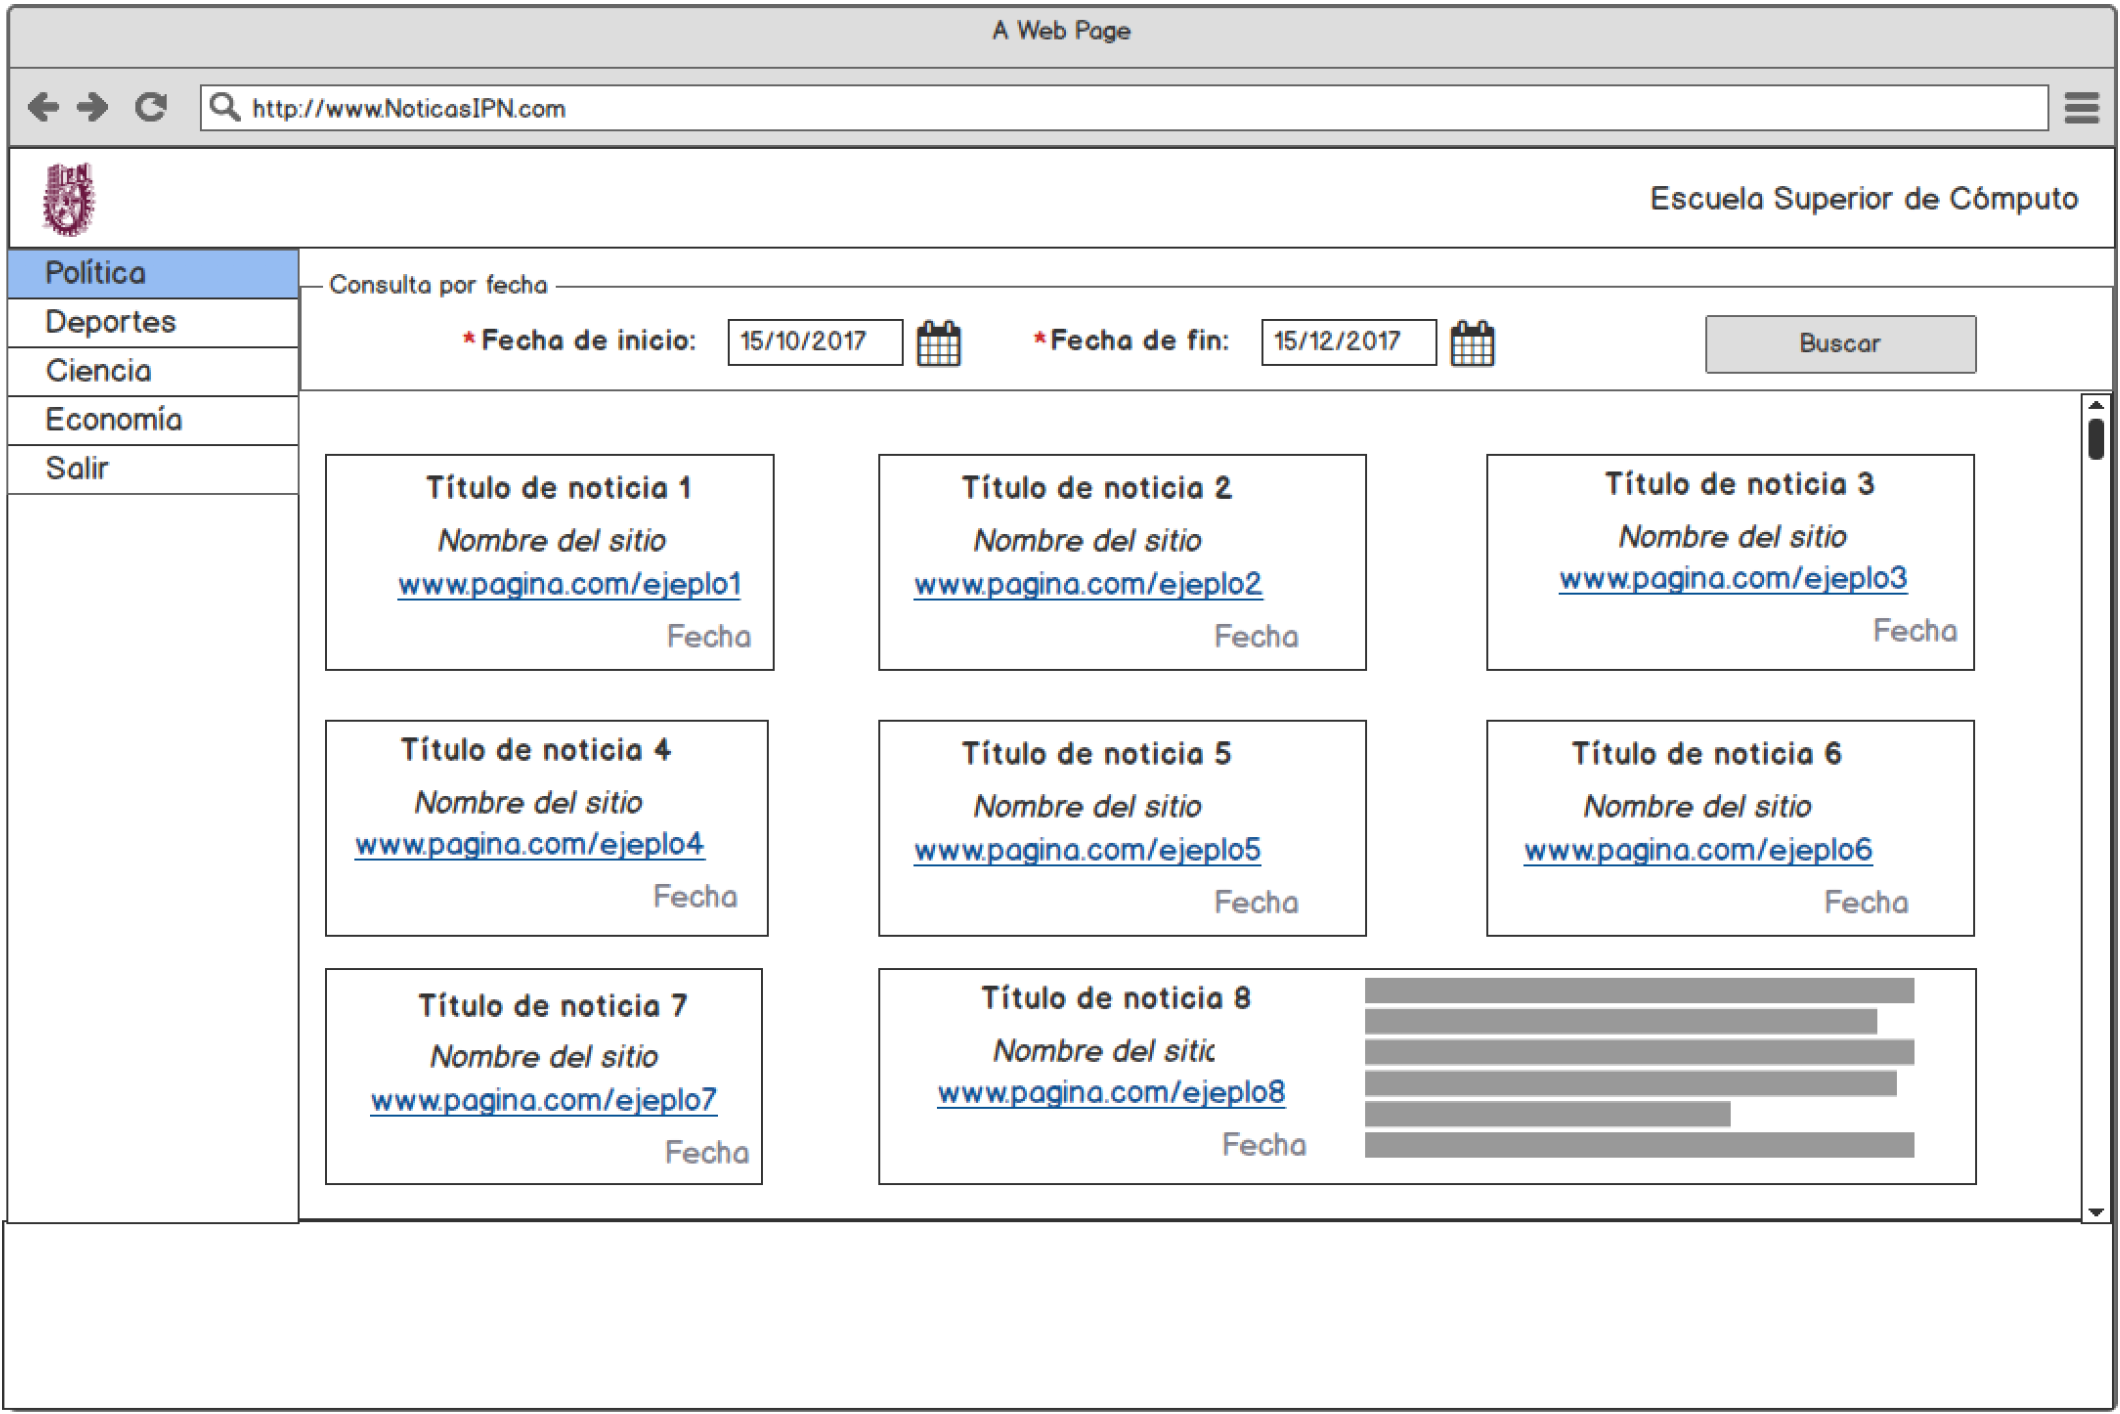
\includegraphics[scale=.3]{imagenes/Pantallas/UI3}
  \caption{Pantalla IU3-Busqueda por fecha}
  \label{fig:IU3}
\end{figure}
\newpage
\subsection{UI4-Página ejemplo}

\Large{\textbf{Objetivo}}\\\\
\normalsize{Texto}\\



\Large{\textbf{Descripción}}\\
\normalsize{Texto}\\


\Large{\textbf{Comandos}}\\
\normalsize{Texto}

\begin{itemize}
	\item Lorem ipsum
	\item Lorem ipsum
	\item Lorem ipsum
\end{itemize}

\Large{\textbf{Referencia}}\\\\
\normalsize{Nombre Caso de uso}

\begin{figure}
  \centering
	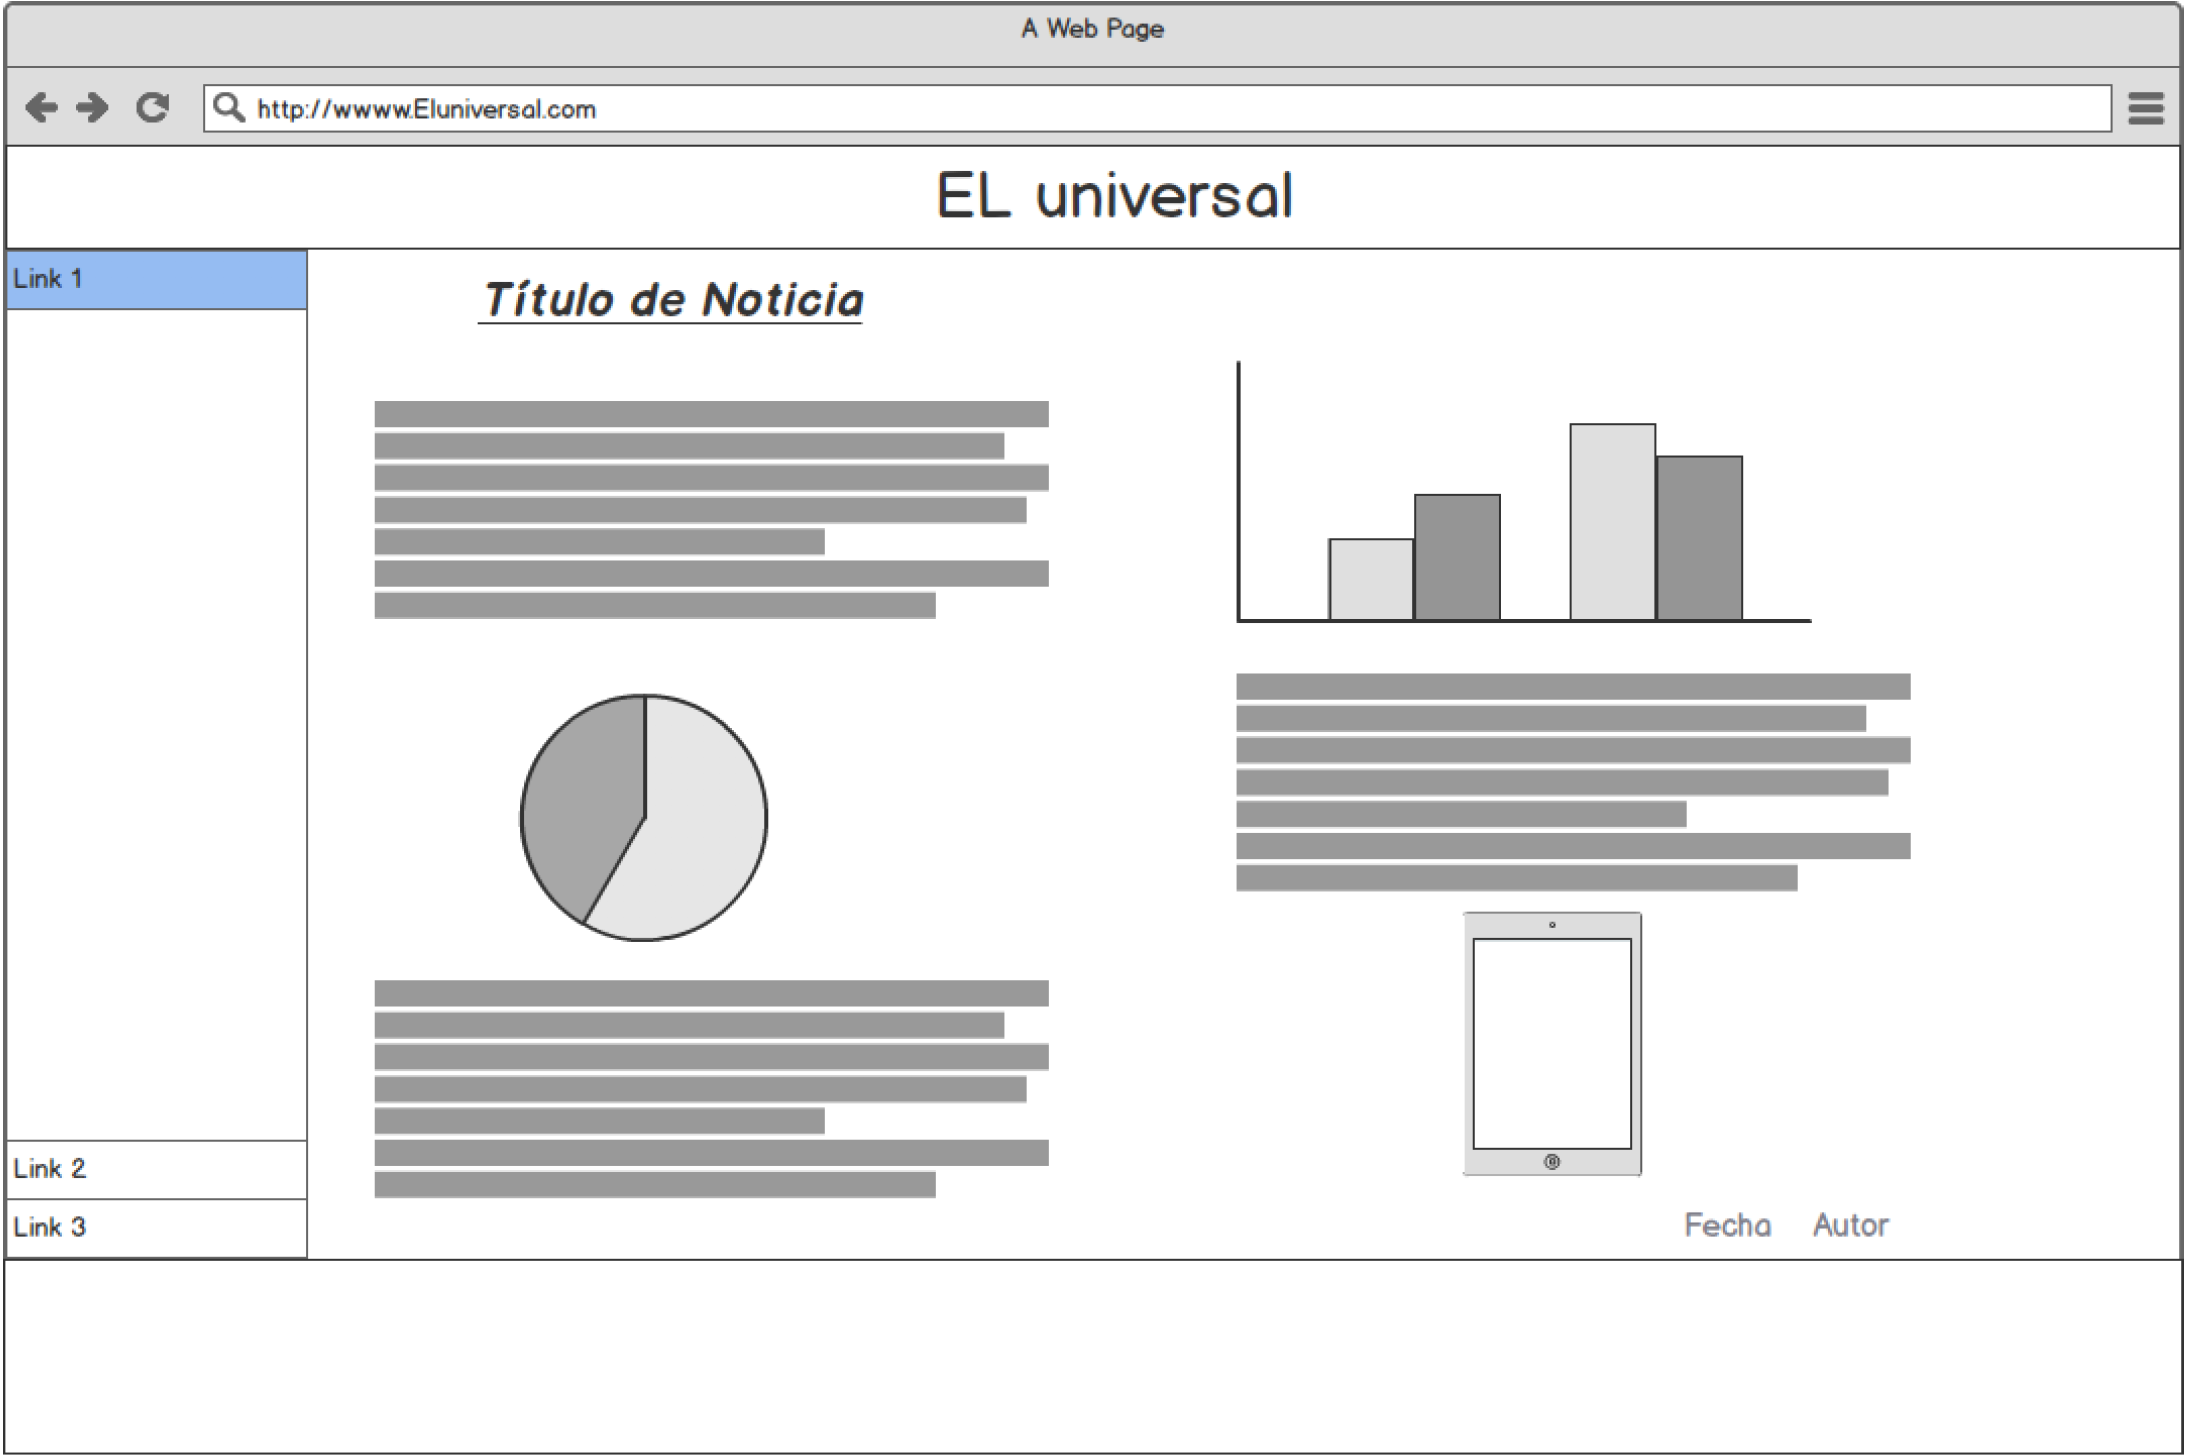
\includegraphics[scale=.3]{imagenes/Pantallas/UI4}
  \caption{Pantalla IU4-Página ejemplo}
  \label{fig:IU4}
\end{figure}
\newpage




